\documentclass[border=4pt]{standalone}

\usepackage[T1]{fontenc}
\usepackage[utf8]{inputenc}
\usepackage{amsmath}
\usepackage{amssymb}
\usepackage{xcolor}
\usepackage{tikz}
\usetikzlibrary{positioning, fit, calc, arrows.meta, backgrounds}

\definecolor{credit}{RGB}{93,170,99}     % credited sub-action (green)
\definecolor{gridc}{RGB}{165,165,165}

\begin{document}

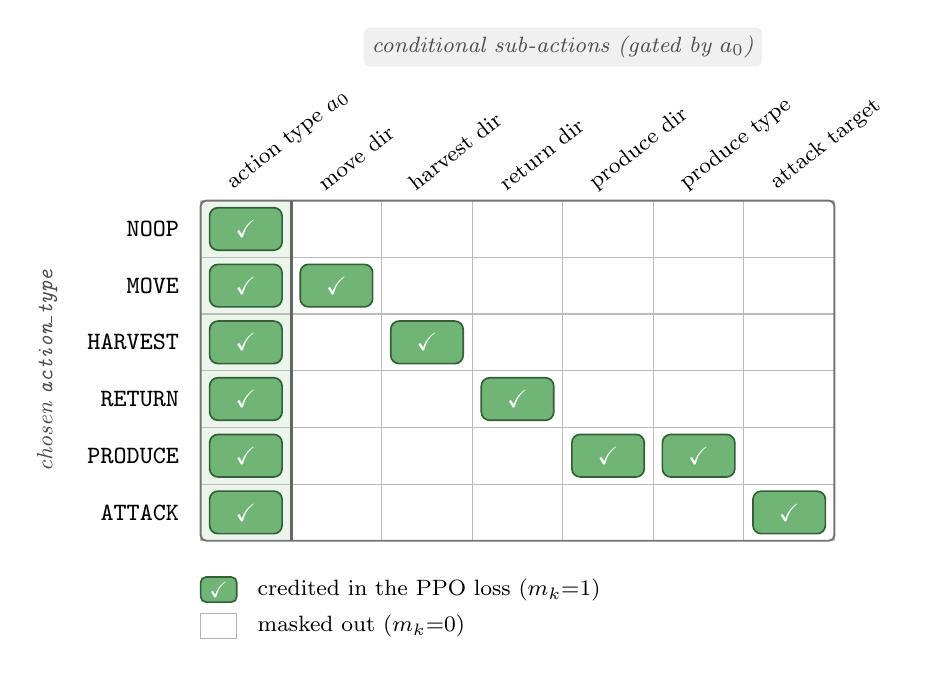
\begin{tikzpicture}[font=\small]

%% ── always-active column highlight (action type is always credited) ──
\begin{scope}[on background layer]
  \fill[credit!12] (0,0) rectangle (1.15,-4.32);
\end{scope}

% geometry: column width 1.15, row height 0.72.
% grid lines fall at multiples of the step from the origin, so we place
% the bounding box at (0,0) and put each cell CENTRE at
%   x = (c+0.5)*1.15 ,  y = -(r+0.5)*0.72   (c = 0..6, r = 0..5).

%% ── credited cells: rounded green chips with a check ─────────────
\foreach \r/\c in {0/0, 1/0,1/1, 2/0,2/2, 3/0,3/3, 4/0,4/4,4/5, 5/0,5/6}{
  \draw[fill=credit!88, draw=credit!55!black, line width=0.6pt, rounded corners=3pt]
    ({(\c+0.5)*1.15-0.46},{-(\r+0.5)*0.72+0.27})
    rectangle
    ({(\c+0.5)*1.15+0.46},{-(\r+0.5)*0.72-0.27});
  \node[white] at ({(\c+0.5)*1.15},{-(\r+0.5)*0.72}) {\bfseries\checkmark};
}

%% ── grid + outer frame ───────────────────────────────────────────
\draw[gridc!75, line width=0.4pt, xstep=1.15, ystep=0.72] (0,0) grid (8.05,-4.32);
\draw[black!55, line width=0.7pt, rounded corners=2pt] (0,0) rectangle (8.05,-4.32);
% separator between the always-active type column and the conditional ones
\draw[black!60, line width=1.1pt] (1.15,0) -- (1.15,-4.32);

%% ── column headers (rotated) ─────────────────────────────────────
\foreach \c/\lab in {0/{action type $a_0$},1/{move dir},2/{harvest dir},3/{return dir},4/{produce dir},5/{produce type},6/{attack target}}{
  \node[rotate=38, anchor=west, font=\footnotesize] at ({(\c+0.5)*1.15-0.30},0.12) {\lab};
}

%% ── conditional-block label ──────────────────────────────────────
\node[font=\footnotesize\itshape, text=black!70, fill=black!6,
      rounded corners=2pt, inner sep=3pt] at (4.60,1.95)
  {conditional sub-actions (gated by $a_0$)};

%% ── row labels (the chosen action type) ──────────────────────────
\foreach \r/\lab in {0/NOOP,1/MOVE,2/HARVEST,3/RETURN,4/PRODUCE,5/ATTACK}{
  \node[anchor=east, font=\ttfamily\small] at (-0.15,{-(\r+0.5)*0.72}) {\lab};
}
\node[rotate=90, font=\itshape\footnotesize, text=black!70] at (-1.95,-2.16)
  {chosen \texttt{action\_type}};

%% ── legend (stacked, left-aligned) ───────────────────────────────
% credited
\draw[fill=credit!88, draw=credit!55!black, line width=0.6pt, rounded corners=2pt] (0,-4.78) rectangle (0.46,-5.10);
\node[white] at (0.23,-4.94) {\footnotesize\bfseries\checkmark};
\node[anchor=west, font=\footnotesize] at (0.60,-4.94) {credited in the PPO loss ($m_k{=}1$)};
% masked
\draw[gridc!85, line width=0.4pt] (0,-5.24) rectangle (0.46,-5.56);
\node[anchor=west, font=\footnotesize] at (0.60,-5.40) {masked out ($m_k{=}0$)};

\end{tikzpicture}

\end{document}
